\subsection{Poiseuille flow}\label{sec:poiseuille}
The domain is a rectangle with $L_x=2$ and $L_y=1$ and constant density and viscosity ($\rho=1$ and $\eta=1$), gravity acceleration $\bm{g}=\bm{0}$ and penalty
parameter $\lambda=10^8$. The grid is composed by $40 \times 20$ elements. Velocity boundary conditions are set to no slip $(\bm{v}=\bm{0})$ at the top and the
bottom, and a parabolic profile is imposed on the sides, with $u=y(1-y)$ and $v=0$. The analytical solution is then given by:
\begin{eqnarray}
u(x,y)&=&y(1-y)\nonumber \\
v(x,y,)&=&0\nonumber \\
p(x,y)&=&2\eta\left(\frac{L_x}{2}-x\right)\nonumber
\end{eqnarray}

The velocity field predicted by the model follows the expected parabolic profile (Fig. \ref{fig:poiseuille}a and Fig. \ref{fig:poi_plot}a) and, in case of the
classic penalty method with no iterations, the pressure is clearly related to the divergence by means of the penalty parameter (Fig. \ref{fig:poiseuille}b and
c and Fig. \ref{fig:poi_plot}b). Fig. \ref{fig:poiseuille}d shows that one Uzawa iteration is sufficient to bring the divergence down to \num{e-15}, with no
correlation with the pressure field. All data can be found at \url{https://github.com/aleregorda/Benchmarks/tree/main/Momentum_equation/Poiseuille%20Flow}.

\begin{figure}
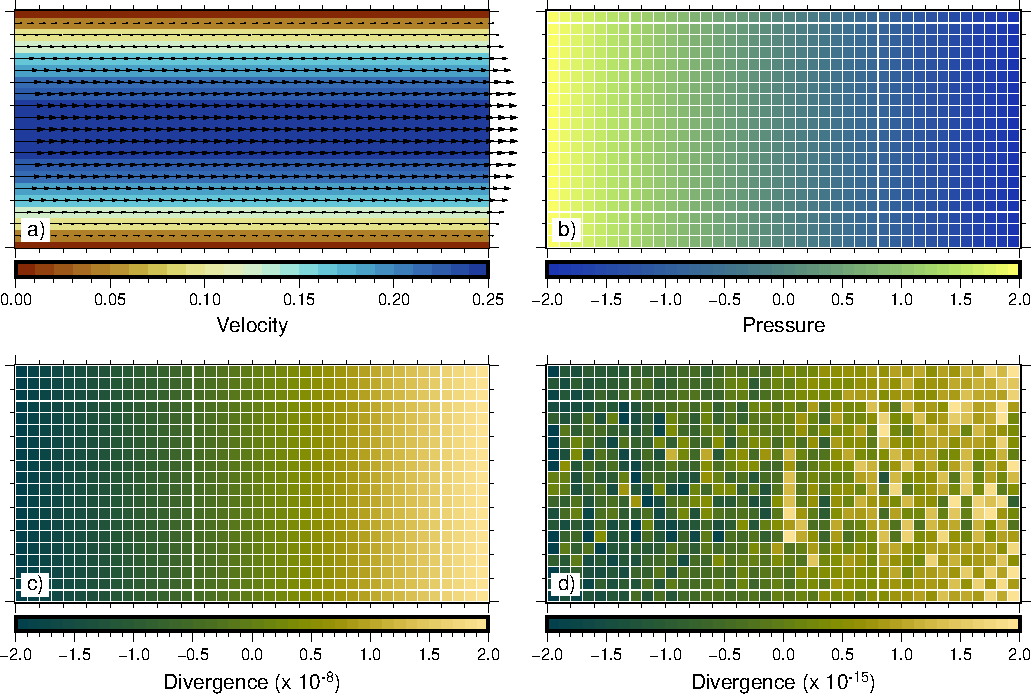
\includegraphics[width=\linewidth]{./Figures/Poiseuille.pdf}
\caption{Velocity field (panel a), pressure (panel b) and divergence velocity of a Poiseuille flow in case of the classic penalty method (no iterations) and
after one Uzawa iteration (panel c and d, respectively).}
\label{fig:poiseuille}
\end{figure}

\begin{figure}
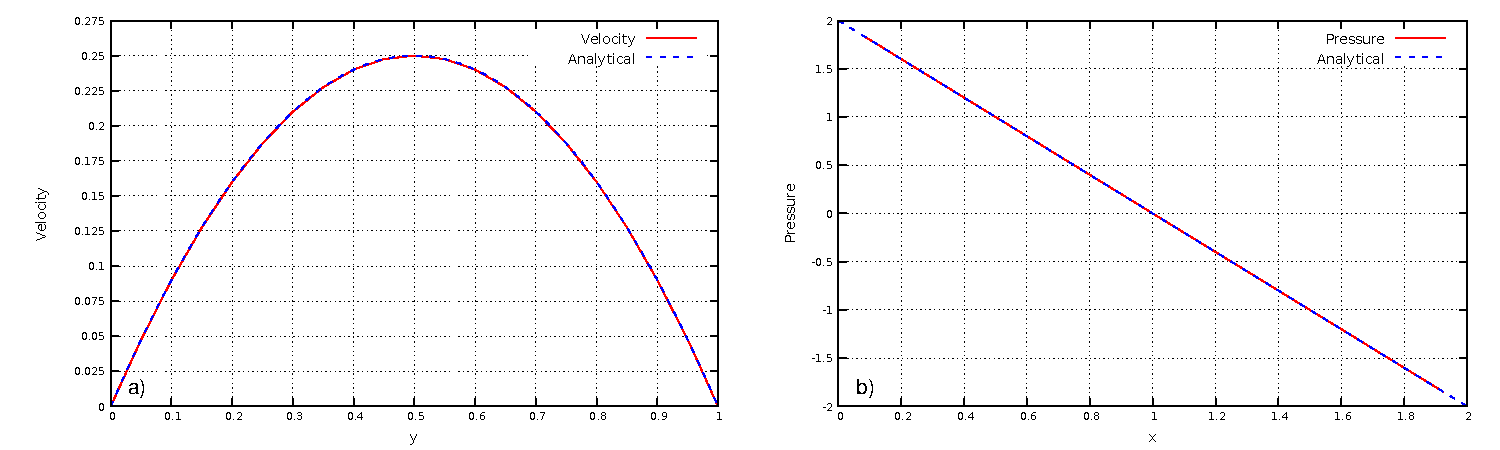
\includegraphics[width=\linewidth]{./Figures/Analytical.pdf}
\caption{Velocity (panel a) and pressure (panel b) field predicted by the model for a Poiseuille flow with respect with their analytical solutions. The
velocity field is plotted as function of the vertical coordinate in $L_x/2$ and the pressure is plotted as function of the x coordinate in $L_y/2$.}
\label{fig:poi_plot}
\end{figure}